% \Image{Capa do livro (; )}{PNLD2022-001-01.png}
% \Image{Ilustração do livro (Acorde/Manuella Silveira; Acorde)}{PNLD2022-001-04.png}
% \Image{Ilustração do livro (Acorde/Manuella Silveira; Acorde)}{PNLD2022-001-05.png}
% \Image{Ilustração do livro (Acorde/Manuella Silveira; Acorde)}{PNLD2022-001-06.png}

\documentclass[11pt]{extarticle}
\usepackage{manualdoprofessor}
\usepackage{fichatecnica}
\usepackage{lipsum,media9}
\usepackage[justification=raggedright]{caption}
\usepackage[one]{bncc}
\usepackage[araucaria]{../edlab}
\usepackage{marginnote}
\usepackage{pdfpages}

\newcommand{\AutorLivro}{Patativa do Assaré}
\newcommand{\TituloLivro}{História de Aladim e a lâmpada maravilhosa}
\newcommand{\Tema}{Diversão e aventura}
\newcommand{\Genero}{Cordel}
%\newcommand{\imagemCapa}{./images/PNLD2022-001-01.jpeg}
\newcommand{\issnppub}{XXX-XX-XXXXX-XX-X}
\newcommand{\issnepub}{XXX-XX-XXXXX-XX-X}
% \newcommand{\fichacatalografica}{PNLD0001-00.png}
\newcommand{\colaborador}{Paulo Pompermaier}

\begin{document}

\title{\TituloLivro}
\author{\AutorLivro}
\def\authornotes{\colaborador}

\date{}
\maketitle

\tableofcontents

\section{Carta ao professor}

Caro professor,

Este material tem a intenção de contribuir para que você consiga desenvolver um trabalho aprofundado com a obra \textit{História de Aladim e a lâmpada mágica} em sala de aula.
Você encontrará informações sobre o autor, sobre o gênero e também 
algumas propostas de trabalho para a sala de aula que você poderá explorar livremente, 
da forma que considerar mais apropriada para os seus estudantes.

Talvez o mais conhecido cordelistas do Brasil, Patativa de Assaré é de importância incontornável. Através de sua extensa obra, o poeta trabalhou com criatividade diversos temas comuns à tradição oral e à literatura de cordel.
Nascido Antonio Gonçalves da Silva, no Cariri, na Serra de Santana, próximo a Assaré,
no Ceará, a 5 de março de 1909, Patativa 
desde menino fazia versos e os apresentava a
quem quisesse ouvir. Só em 1956 seus poemas apareceriam em livro, com a edição
pela Borsoi, do Rio de Janeiro, do belo \textit{Inspiração Nordestina}. O
sucesso de grande público, contudo, viria pouco depois, em 1964, com a gravação
em disco de ``A triste partida'', poema musicado pelo Rei do Baião, Luiz
Gonzaga. Poeta de genuína inspiração popular, Patativa do Assaré tornou-se
sinônimo de poesia popular no país, tendo lançado, em sua longa vida de quase
um século, uma dezena de livros e discos com seus poemas, além de inúmeros
folhetos avulsos de cordel. 

No caso de \textit{História de Aladim e a lâmpada mágica}, trata-se de um poema em cordel inspirado na clássica história do \textit{Livro das mil e uma noites}.
Além da história saborosa, cheia de peripécias e aventuras, a obra é importante pois introduz o aluno no universo do cordel, uma das maiores expressões da cultura popular oral brasileira. E o faz através de personagens e acontecimentos narrados em Bagdá, capital do Iraque, na época das narrativas mágicas do \textit{Livro das mil e uma noites}. Esse salto temporal e espacial coloca o estudante diretamente em contato com uma cultura muito distante da sua, evidenciando a importância das diferentes expressões culturais para a formação de uma obra artística e, de forma geral, para a nossa própria sociedade globalizada. Além, é claro, de expressar uma das características fundadoras da literatura de cordel: a influência dos mitos, lendas e personagens medievais (europeus ou não) para a cultura popular brasileira. 
Pela presença do mágico e fantástico, ademais, o poema torna-se ainda mais apelativo e chamativo para um público juvenil, sendo uma excelente porta de entrada para habituar os jovens à prática da leitura e introduzi-los em uma rica vivência literária.

Ao longo do manual, todos esses aspectos serão explorados e relacionados a sugestões de atividades. Com isso, objetiva-se oferecer algumas ideias e inspirações para um trabalho que pode ser desenvolvido tanto a curto, quanto a médio e longo prazo. Sinta-se à vontade para personalizar a aula e torná-la sua, aplicando seus conhecimentos, sua 
personalidade e aproveite para fortalecer seu vínculo com a turma.
Boa aula!

\section{Sobre o livro}
A narrativa se passa em Bagdá, na época de prosperidade e riqueza dessa cidade.
Aladim, filho travesso e preguiçoso de uma viúva, decide trabalhar para ajudar a mãe.
Enquanto busca por trabalho, chega à cidade o “Feiticeiro Africano”, personagem misterioso que está à procura da lâmpada mágica escondida em uma gruta. No entanto, somente uma pessoa que não conhece a lâmpada pode pegá-la, e então o Feiticeiro persuade Aladim a lhe ajudar, prometendo-lhe riquezas e felicidade.

A gruta está localizada em um vale no deserto, entre dois morros, na qual o jovem Aladim deveria entrar para encontrar a lâmpada. Com medo da escuridão, o Feiticeiro empresta-lhe um anel mágico, que o iria proteger de qualquer perigo. O Feiticeiro, no entanto, é grosseiro e maltrata Aladim que, por isso, após encontrar a lâmpada, hesita em entregá-la ao Feiticeiro. Sentido-se traído, ele fecha a porta da gruta e mantém Aladim preso lá dentro, onde permanece por três dias. Desesperado, reza por salvação e, ao esfregar as mãos na prece, o anel mágico se mexe e invoca um gênio mágico.

O primeiro pedido do garoto ao gênio é voltar para a casa da mãe, em Bagdá. O pedido é prontamente atendido. A mãe, desconfiada da história fantástica, esfrega a lâmpada que estava com Aladim e novamente aparece um gênio. Aladim pede-lhe sustento e recebe uma rica prataria e fartura de alimentos. Graças ao gênio, Aladim e sua mãe vivem de maneira folgada por alguns anos, até Aladim apaixonar-se pela princesa Clarice, filha do sultão de Bagdá. O jovem tem um plano para conquistar a mão da princesa: pede à sua mãe que se dirija ao palácio com as riquezas que trouxera da caverna, para propor ao sultão o casamento dos jovens. O sultão, no entanto, exige mais riquezas e quarenta escravos como dote para o casamento. Com a ajuda do gênio, consegue o dote solicitado e casa-se, por fim, com Clarice.

Enquanto isso, ao saber que Aladim o lograra e escapara da grupa, o Feiticeiro trama uma vingança contra o recém-casado. Disfarçado de um pobre vendedor de lâmpadas, o necromante engana Clarice e consegue roubar o item mágico. Usa, então, a lâmpada para transferir o palácio de Aladim e todos que nele estacam para seus domínios, exceto o sultão e Aladim, que tinham ido caçar. Condenado à morte pelo desaparecimento da princesa, Aladim consegue escapar graças ao anel encantado, transferindo-se ao palácio nas terras do Feiticeiro, que pretendia casar-se com Clarice. Com seu auxílio, Aladim envenena o raptor e transfere o palácio ao seu lugar original, onde vivem felizes para sempre. No final, a moral da história mostra como a ambição contamina o coração dos homens e os faz cometer maldades, que, no entanto, podem se voltar contra eles. Como nos versos finais, a ambição ``traz consigo a maldição / amamentando a desgraça / tira o dinheiro do nobre / ilude a gana do pobre / vê do indigente o cobre / a ambição onde passa''.


\reversemarginpar
\marginparwidth=5cm

%\marginnote{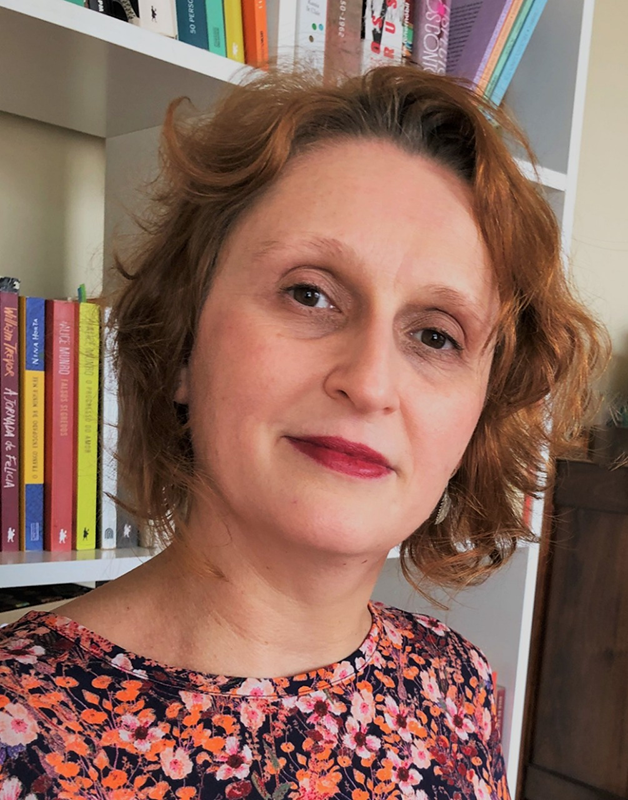
\includegraphics[width=\marginparwidth]{./images/PNLD2022-001-02.png}\\
%A autora Camila Werner (Arquivo pessoal)}


\section{Sobre o autor}


%532 caracteres
\paragraph{O autor}
Antonio Gonçalves da Silva, o Patativa do Assaré, foi um dos mais importantes
poetas brasileiros. Nascido no Cariri, na Serra de Santana, próximo a Assaré,
no Ceará, a 5 de março de 1909, desde menino fazia versos e os apresentava a
quem quisesse ouvir. Só em 1956 seus poemas aparecereiam em livro, com a edição
pela Borsoi, do Rio de Janeiro, do belo \textit{Inspiração nordestina}. O
sucesso de grande público, contudo, viria pouco depois, em 1964, com a gravação
em disco de ``A triste partida'', poema musicado pelo Rei do Baião, Luiz
Gonzaga. Poeta de genuína inspiração popular, Patativa do Assaré tornou"-se
sinônimo de poesia popular no país, tendo lançado, em sua longa vida de quase
um século, uma dezena de livros e discos com seus poemas, além de inúmeros
folhetos avulsos de cordel. De sua obra, destacam"-se os livros
\textit{Inspiração nordestina} (1956), \textit{Cante lá que eu canto cá}
(1978), \textit{Ispinho e fulô} (1988), \textit{Balceiro} (1991), \textit{Aqui
tem coisa} (1994) e \textit{Digo e não peço segredo} (2001); e os discos
\textit{Poemas e canções} (1979), \textit{A terra é naturá} (1981) e
\textit{Canto nordestino} (1989). Doutor \textit{honoris causa} em diversas
universidades, objeto de teses, filmes e peças, a voz da ave canora que lhe deu
nome, a patativa, ainda será ouvida por muitos e muitos anos em qualquer canto
do Brasil. Patativa morreu aos 93 anos em sua casa em Assaré.

Além de poeta extremamente interessante nos causos, histórias e fatos de sua terra, Patativa do Assaré também cantou muito sobre a política e a situação de seu povo, engajando"-se em debates como a reforma agrária.
Nas palavras do próprio poeta:

\begin{quote}
Eu sou um caboclo roceiro que, como poeta, canto sempre a vida do
povo. O meu problema é cantar a vida do povo, o sofrimento do meu
Nordeste, principalmente daqueles que não têm terra, porque o ano
presente, esse ano que está se findando, não foi uma seca, podemos dizer
que não foi a seca. Lá pelo interior, mesmo no município de Assaré, lá
no Assaré, tem duas frentes de serviço, com muita gente. Mas naquela
frente de serviço nós podemos observar que é só dos desgraçados que
não possuem terra. Os camponeses que possuem terra não sofrem estas
consequências e não precisam recorrer ao trabalho de emergência, como
os agregados e esses outros desgraçados trabalham na terra dos patrões.
E é isso que eu mais sinto: é ver um homem que tanto trabalha, pai de
família e não possui um palmo de terra. É por isso que é preciso que
haja um meio da reforma agrária chegar, uma reforma agrária que chegue para o povo que não tem terra.

E esta luta pela reforma agrária e pelo sindicato dos camponeses, mas o
verdadeiro sindicato conduzido pelos próprios camponeses, procurando,
reivindicando os seus direitos, é preciso que continue até chegar o
tempo do camponês sofrer menos do que vem sofrendo. Precisa fazer como
eu digo nos meus versos ``Lição do Pinto'', pois o pinto sai do ovo
porque trabalha. Ele belisca a casca do ovo, rompe e sai. É assim que o
povo também deve fazer, unido sempre, trabalhando.\footnote{Depoimento concedido a Rosemberg
Cariry, no Crato, em 1979.}
\end{quote}

\paragraph{A obra de Patativa do Assaré}
Inserida no contexto sertanejo, a obra de Patativa do Assaré é influenciada pela tradição medieval, como a arte dos trovadores, que viria a influir na formação da poesia de cordel, marcada pela figura dos repentistas, violeiros e cantadores.
Cantando os sofrimentos e desgraças, mas também as alegrias da população nordestina do sertão, é forçoso reconhecer Patativa do Assaré como um dos maiores representamtes da literatura de cordel. Nas palavras de Sylvie Debs, estudiosa da obra do poeta:

\begin{quote}
Testemunha então de um modo de vida, mas também reivindicação de valores
próprios, elaboração de uma identidade. Por isso, ele é apresentado como o
“verdadeiro, autêntico e legítimo intérprete do sertão”.\footnote{ Plácido Cidade
Nuvens, \textit{Patativa e o universo fascinante do sertão}, p. 15.} Com
efeito, uma das dimensões mais marcantes da obra de Patativa do Assaré é a
preocupação de descrever a vida cotidiana do sertão e, com esse testemunho,
protestar o reconhecimento da dignidade, da integridade e da modéstia do
camponês sertanejo, em oposição à arrogância do cidadão urbano ou do brasileiro
do Sul. Parece que a afirmação de sua própria identidade passa mais
frequentemente pelo confronto com o outro, como chama atenção o título da
compilação: \textit{Cante lá que eu canto cá}. Esta última, composta a partir de uma
seleção de textos feita pelo próprio autor com a intenção de definir suas
preferências literárias, traz o seguinte subtítulo: Filosofia de um trovador
nordestino. É, portanto, referindo"-nos de uma só vez ao conjunto dos poemas
publicados e à vida de Patativa do Assaré que tentaremos depreender as
características próprias da sua obra.\footnote{\textsc{debs}, Sylvie. ``Introduçã''. In: \textsc{assaré}, Patativa do. \textit{Cordel na escola}. São Paulo: Hedra, 2000, p.\,14.}
\end{quote}

Nas primeiras obras do poeta, fruto de improvisações e encomendas, ressaltam"-se os traços lúdicos e comemorativos. São poemas de circunstâncias, ligados aos acontecimentos sociais e religiosos, como festas de santos, casamentos, aniversários e outros acontecimentos com relação direta com o presente.
É uma poesia, portanto, que está fortemente inserida na vida da comunidade e dela participa.

Como ressalta Sylvie Debs, a marca da oralidade, inserida nesse contexto comunitário, era tão forte que as primeiras compilações de sua poesia saíram com alguns aparatos para orientar o leitor nesse novo vocabulário: ''A marca oral e regional era tão intrínseca à primeira compilação que foi
publicada com um “Elucidário” que propunha três esclarecimentos diferentes ao
leitor: uma simples restituição fonética (\textit{biête} por bilhete ou \textit{muié} por mulher), uma correspondência referencial (cão por diabo) e uma explicação denotativa (tipoia: rede pequena, rede velha)''.\footnote{Ibid., p.\,15.}

Outra marca significativa da oralidade, ainda na análise de Debs, é a forte presença da função conotativa da linguagem:

\begin{quote}
interpelação do ouvinte como
\textit{Cante lá que eu canto cá}, interrogações como “Você se lembra?”, “Seu Dotô me
conhece?”, destinação como “Ao leitor”, “Aos poetas clássicos”, “À minha esposa
Belinha”. Da mesma forma, os primeiros versos de seus poemas instauram,
geralmente, o ritual discursivo, seja como forma de indagação: “Querem saber
quem eu sou?” (\textit{Aqui tem coisa}, p. 63); seja sob forma de oração: “Quero que me dê licença
para uma história contá.” (\textit{Cante lá que eu canto cá}, p. 47); seja por uma saudação: “Boa noite, home
e menino e muié dêste lugá.” (\textit{Inspiração nordestina}, p. 27); seja ainda por uma ordem: “Vem cá,
Maria Gulora, escuta, que eu vou agora uma coisa te contá.” (\textit{Idem}, p. 47). Enfim,
a invocação do interlocutor abre diversos poemas: as formas mais utilizadas são
“Seu Moço” (\textit{Idem}, pp. 19, 51, 99) e “Seu Dotô” (\textit{Idem}, pp. 60, 66 e 69). Encontram-se
variantes sob a forma de “Meu filho querido” (\textit{Idem}, p. 132), “Meu amigo” (\textit{Idem}, p.
209), “Minha gente” (\textit{Idem}, p. 206), “Sinhô Dotô”
(\textit{Idem}, p. 203).\footnote{Ibidem.}
\end{quote}

Através dessa referencialidade a pessoas e circunstâncias de seu entorno, percebe"-se na poesia de Patativa do Assaré o forte tom familiar e a relação de vizinhança que está implicada em seus poemas, marcas de um autor enraizado ao seu meio:

\begin{quote}
Esses termos de
endereçamento traduzem ao mesmo tempo o respeito de uma hierarquia social
estrita, em uma sociedade onde a taxa de analfabetismo é elevada. O poeta, como
personagem familiar, é originário do mesmo meio, dirigindo-se em pé de igualdade
a seus interlocutores, seja ao mais rico, ao mais poderoso ou ao mais diplomado,
pedindo licença para contar uma história simples à sua maneira -- último
elemento enfim, todavia essencial, o próprio poeta Patativa do Assaré. Não
havendo jamais escrito texto algum e dotado de uma notável capacidade de
memorização (é capaz de recitar qualquer uma de suas composições, qualquer seja
sua antiguidade), ele continua a praticar a improvisação em todas as
circunstâncias.\footnote{Ibidem.}
\end{quote}


\paragraph{O ilustrador}
Fernando de Almeida nasceu em Batatais, interior de São Paulo, em 1973. Formado em Arquitetura pela \textsc{fau-usp}, trabalha como ilustrador e designer gráfico.
Já ilustrou páginas da \textit{Folha de São Paulo}, \textit{\textsc{tam} Magazine} e revista \textit{Bravo!} entre outras. Faz, junto com outros amigos ilustradores, a revista coletiva \textit{Charivari}. Gosta de aquários, fuscas antigos, de sua mulher Cristiana, do seu filho Martim e dos seus amigos.


\section{Sobre o gênero}

%55 caracteres
\paragraph{O gênero} O gênero deste livro é \textit{poesia de cordel}. 


Para uma primeira definição de poesia enquanto gênero literário, poder"-se"-ia recorrer à definição do professor Domingos Paschoal Cegalla, para quem ``poesia é a linguagem subjetiva, carregada de emoção e sentimento, com ritmo melódico constante, bela e indefinível como o mundo interior do poeta visa a um efeito estético''.\footnote{\textsc{cegalla}, Domingos Paschoal. \textit{Novíssima Gramática da Língua Portuguesa}. São Paulo: Companhia Editora Nacional, 2008, p.\,640}

Aprofundando um pouco essa definição, o crítico Antonio Candido expande a definição de poesia ao diferenciá"-la do verso.
Para o crítico, a poesia enquanto ato criador do artista independe da forma métrica do verso, que passa a ser apenas um dos registros possíveis do poético:

\begin{quote}
A poesia não se confunde necessariamente com o verso, muito menos com o verso metrificado. Pode haver poesia em prosa e poesia em verso livre. [\ldots]
Pode ser feita em verso muita coisa que não é poesia.\footnote{\textsc{candido}, Antonio. \textit{O estudo analítico do poema}. São Paulo: Terceira leitura, 1993, p.\,13--14.}
\end{quote}

Delineada, de forma breve e geral, a forma poética, pode"-se pensar agora em seus três gêneros básicos: lírico, épico e dramático.
Para o crítico Anatol Rosenfeld, a lírica é o gênero mais subjetivo, no qual uma voz central exprime um estado de alma traduzido em orações poéticas.
Seria a expressão de emoções e experiências vividas, ``a plasmação imediata das vivências intensas de um Eu no encontro com o mundo, sem que se interponham eventos distendidos no tempo (como na Épica e na Dramática)''.\footnote{\textsc{rosenfeld}, Anatol. \textit{O teatro épico}. São Paulo: Perspectiva, 2006, p.\,22.}

Devido a essa característica central da lírica, a expressão de um estado emocional, Rosenfeld considera que o eu"-lírico, nesse gênero, não se delineia enquanto um personagem. Embora possa evocar personagens e narrar acontecimentos, a lírica entendida enquanto gênero puro afasta"-se sobremaneira da apreensão objetiva do mundo, que não existe independente da subjetividade intensa que o apreende e exprime. Assim, na lírica prevalece a fusão entre o sujeito e o objeto, que serve mais a realçar os estados profundos de alma do poeta.
Sobre os aspectos formais do gênero, Rosenfeld nota:

\begin{quote}
À intensidade expressiva, à concentração e ao caráter ``'imediato'' do poema lírico, associa"-se, como traço estilístico importante, o uso do ritmo e da musicalidade das palavras e dos versos. De tal modo se realça o valor da aura conotativa do verbo que este muitas vezes chega a ter uma função mais sonora que lógico"-denotativa. A isso se liga a preponderância da voz do presente que indica a ausência de distância, geralmente associada ao pretérito. Este caráter do imediato, que se manifesta na voz do presente, não é, porém, o de uma atualidade que se processa e distende através do tempo (como na Dramática) mas de um momento ``eterno''.\footnote{Ibidem, p.\,23.}
\end{quote}

No caso específico da poesia de cordel, dizem os especialistas, é uma poesia escrita para
ser lida, enquanto o repente ou o desafio é a poesia feita oralmente, que mais tarde pode
ser registrada por escrito. Essa divisão é muito esquemática. Por exemplo, o
cordel, mesmo sendo escrito e impresso para ser lido, costumava ser lido em
volz alta e desfrutado por outros ouvintes além do leitor. A poesia popular,
praticada principalmente no Nordeste do Brasil, tem muita influência da
linguagem oral, aproveita muito da língua coloquial praticada nas ruas e na
comunicação cotidiana. 

Naturalmente, portanto, pode"-se considerar a poesia narrativa do cordel uma
forma de poesia mais compartilhada e desfrutada coletivamente, o que dá também
uma grande ressonância social. Muitos dos temas do cordel são originários das
tradições populares e eruditas da Europa medieval e moderna. Outros temas são
retirados de tradições orientais, como neste \textit{História de
Aladim e a lâmpada maravilhosa}. O personagem Aladim pertence ao \textit{Livro das mil
e uma noites}, um dos famosos conjuntos de histórias de todos os tempos. Também
encontramos temas retirados das novelas de cavalaria medievais e das narrativas
bíblicas. Ao lado destes temas mais literários, encontram"-se os temas locais,
quase sempre narrados na forma de crônicas de coisas realmente acontecidas,
como em outro famoso cordel de Patativa intitulado  “Padre Henrique e o dragão da maldade”, que fala de um causo verídico e contemporâneo ao poeta. Também há, entre sua profícua produção literária, as histórias
fantásticas, que se valem das tradições semirreligiosas, ligadas à experiência
com o mundo espiritual. 

Os grandes poemas de cordel são perfeitamente metrificados e rimados. A métrica
e a rima são recursos que favorecem a memorização e tradicionalmente se costuma
dizer que são resquícios de uma cultura oral, na qual toda a tradição e
sabedoria são sabidas de cor.  


\paragraph{O sertão geográfico e cultural}

O sertão tem mitos culturais próprios. Contemporaneamente, o sertão evoca
principalmente o sofrimento resignado daqueles que padecem a falta de chuva e
de boas safras na lavoura. Evoca a experiência histórica de uma região
empobrecida, embora tenha sido geradora de riquezas, como o cacau e cana de
açúcar, ambos bens muito valiosos. 

O sertão formou também o seu imaginário por meio de grandes personalidades e
uma pujante expressão artística. Além do cordel, o sertão viu nascer ritmos tão
importantes quanto o forró e o baião. Produziu artistas tão expressivos quanto
Luiz Gonzaga, grande cantor da vida do sertanejo em canções como “Asa branca”.
Um escultor como Mestre Vitalino criou toda uma tradição de representação da
vida e dos hábitos sertanejos em miniaturas de barro. A gravura popular, que
sempre acompanha os folhetos de cordel, também floresceu em diversos pontos e
ficou mais famosa em Juazeiro do Norte, no Ceará, e em Caruaru, no estado de
Pernambuco. 

Dentre os grande mitos do sertão, está certamente o do cangaço com seu líder
histórico, mas também mítico, Virgulino Ferreira, o Lampião. Até hoje as
opiniões se dividem: para alguns foi uma grande homem, para outros um bandido
impiedoso. 

Uma figura muito presente na cultura nordestina é o Padre Cícero Romão,
considerado beato pela Igreja Católica. Consta que teria feito milagres e
dedicado sua vida aos pobres. 

\paragraph{Variação linguística}

A linguística moderna usa o termo “idioleto” para marcar grupos distintos no
interior de uma língua. Um idioleto pode ser a fala peculiar de uma região, de
um grupo étnico ou de uma dada profissão. 

Uma das grandes forças da poesia popular do Nordeste se origina em sua forma
muito própria de falar, com um ritmo muito diferente dos falares do sul, e
também muito diferentes entre si, pois percebe"-se a diferença entre os falares
de um baiano, um cearense e um pernambucano, por exemplo.

Além desse aspecto rítmico, quase sempre também há palavras peculiares a certas
regiões. 


\section{Atividades}

\subsection{Pré-leitura}

\subsubsection{Atividade 1}

\BNCC{EF15AR03}
\BNCC{EF15LP15}

\paragraph{Tema} A literatura de cordel e suas características estéticas e culturais.

\paragraph{Conteúdo} Introduzir a literatura de cordel aos estudantes, apresentando diferentes títulos e incentivando que busquem características semelhantes que permitam caracterizar determinadas obras como literatura de cordel.

\paragraph{Objetivo} Fornecer aos estudantes subsídios para pensar as distintas matrizes artísticas que compõem a cultura brasileira, com enfoque nas características e peculiaridades da literatura de cordel.

\paragraph{Justificativa} A literatura de cordel é um patrimônio da cultura brasileira. Publicada no formato de folheto, geralmente traz para o universo escrito casos e histórias já comuns na tradição oral popular. Entre suas características típicas estão a construção do texto por meio de rimas e a utilização de gravuras, normalmente impressas por meio da xilogravura, que caracterizam as obras com seu tracejado muito próprio. Conhecer a literatura de cordel, portanto, não é apenas entrar em contato com uma importante matriz cultural do Nordeste, mas com uma das mais importantes e características correntes artísticas que constituem o Brasil.

\paragraph{Metodologia} Para uma primeira aproximação da obra poética de Patativa do Assaré, recomenda-se ao professor explorar o formato do folheto de cordel e suas principais características, familiarizando os alunos no universo do cordel no qual estão entrando. 
Para uma primeira abordagem, podem-se levantar questões que instiguem os alunos a pensar nas peculiaridades do cordel.
Algumas perguntas para orientar essa primeira atividade poderiam ser:

\begin{itemize}
\item Alguém já viu ou ouviu falar sobre a literatura de cordel?

\item Se sim, quais características conseguem observar?

\item Se não, o que vem à cabeça ao pensar em ``cordel''?

\item Alguém já ouviu falar no Patativa do Assaré?

\item De qual região do país imaginam que vem a literatura de cordel?
\end{itemize}


Após verificar o conhecimento prévio que os alunos têm sobre o cordel, comece a explorar alguns temas e características comuns a essa literatura. Pode-se projetar na sala algumas imagens de diferentes cordéis, do modo como tipicamente são dispostos nas feiras, das xilogravuras que acompanham os poemas etc. Outra opção é levar alguns cordéis para os alunos lerem e manusearem na sala, pensando-se que, atualmente, muitas bancas e jornaleiros vendem cordéis a um baixo custo.
Concomitante à exposição imagética dos cordéis, fale sobre suas principais características, tais como: o uso de xilogravuras e a forma de talhar o desenho na matriz de madeira; a relação do cordel com a oralidade; a composição rimada e sua relação com a memorização da história; os temas, personagens e enredos frequentes a essa literatura; o papel dos cordelistas na cultura nordestina etc.
Após essa introdução, converse com os alunos sobre as informações novas que aprenderam e levante um debate em torno de alguns pontos centrais, tais como:

\begin{itemize}
\item Identificar o folheto de cordel e suas características;

\item Diferenciar um folheto de cordel e um livro;

\item Aproximar o poema do folheto e a fala;

\item Identificar quais são as histórias típicas do folheto de cordel;

\item Perceber as características regionais do folheto de cordel.
\end{itemize}

Posteriormente, o professor pode coletar essas informações junto aos alunos e abordá-las durante as aulas sobre o livro. Assim, relaciona-se o cordel de Patativa do Assaré trabalhado em sala com as características estruturais que fazem do poema de Patativa um cordel, apesar de apresentar um formato diferente do cordel tradicional.


%Foto : “Legenda”: imagens de Bagdá ou imagens associadas à narrativa: a lâmpada de azeite usada para iluminar; imagens de folhetos de cordel à venda, nos cordéis;

\paragraph{Tempo estimado} Duas aulas de 50 minutos.


\subsubsection{Atividade 2}

\BNCC{EF02GE04}
\BNCC{EF03GE02}

\paragraph{Tema} Relacionando a literatura à geografia: o mundo árabe.

\paragraph{Conteúdo} Explorar a relação da história de Patativa de Assaré com a tradição literária árabe, explorando os hábitos, características e particularidades de Bagdá, onde a história se passa.

\paragraph{Objetivo} Aprofundar a compreensão geográfica do estudante a partir da literatura. Mostrar como diferentes culturas se misturam e atravessam na tradicional contação de histórias dos cordelistas. 

\paragraph{Justificativa} Como bem demonstrou o escritor paraibano Ariano Suassuna com sua pesquisa armorial, a cultura nordestina é fortemente influenciada por mitos, lendas e folclores medievais europeus. Com a colonização, muitos elementos formadores do caldo cultural medieval foram importados para a colônia portuguesa e, como eram transmitidos oralmente, aqui se continuou essa tradição. Cavaleiros, criaturas mágicas, feiticeiros e bobos visionário, típicos das lendas medievais, abundam também nas narrativas dos cordéis, misturados às crenças, personagens e tradições locais. A cultura árabe, igualmente, participa desse ambiente cultural, afinal a Península Ibérica passou por séculos de domínio mouro e, mesmo após a fundação de Portugal pelo rei Afonso Henriques, os costumes e tradições desenvolvidos por séculos naquele território não foram extinguidos pela ocupação portuguesa, mas misturaram-se à vida cultural, culinária, afetiva etc. portuguesa.

Esse é, precisamente, o caso da história de Aladim e a lâmpada mágica: originalmente, é uma história coletado no famoso \textit{Livro das mil e uma noites}, o principal compêndio de narrativas e mitos do mundo árabe. A partir da obra de Patativa do Assaré, portanto, coloca-se uma oportunidade para introduzir o aluno na cultura de tão distante região, aprofundando sua apreensão sobre a obra de Patativa do Assaré e sobre as diversas culturas que se cruzam e entrelaçam na criação artística.

\paragraph{Metodologia} O poema de Patativa do Assaré se passa em Bagdá, atual capital do Iraque. O educador pode, inicialmente, projetar imagens da cidade em sala de aula, mostrando suas construções históricas, as mesquitas, vestimentas etc. É interessante, igualmente, projetar um mapa, ou usar um mapa-múndi de papel, para mostrar a localização do Iraque e de Bagdá no globo terrestre. Posteriormente, essa apresentação pode ser explorada com o livro em mãos, pois as ilustrações retratam traços característicos do Oriente: as vestimentas das personagens, compostas de burcas, turbantes, coletes, gorro Kufi etc.; as construções com seus ladrilhos coloridos e as características janelas, cúpulas e abóbodas em estilo árabe; a forte presença de regiões desérticas na narrativa etc.

Após essa breve apresentação de Bagdá e algumas características dos povos árabes, converse com os alunos sobre as semelhanças e diferenças que observam entre o que aprenderam e a vida no Brasil. 
Pode-se fazer perguntas como:

\begin{enumerate}
\item Quais diferenças vocês percebem entre essa terra que acabaram de conhecer e o Brasil?

\item Como vocês acham que é a vida das pessoas lá? 

\item Se fôssemos falar do Brasil para uma pessoa que nunca veio para cá, quais características vocês ressaltariam?

\item Quais elementos ilustram melhor nosso país?

\end{enumerate}

A partir das repostas dos alunos, aconselha-se a ir se aproximando da obra, facilitando a introdução da atividade de leitura. Fale um pouco sobre a lenda do Aladim, o uso da lâmpada de azeite para iluminar quando não havia eletricidade, o mito do gênio que realiza três desejos e pergunte se alguém já conhece a história do Aladim.

Como os alunos já foram introduzidos à literatura de cordel na primeira atividade, nesse momento pode-se relacionar mais intimamente a cultura árabe com a cultura nordestina, levantando hipóteses com os alunos que expliquem o uso de uma lenda moura por um poeta nordestino. A riqueza da cultura, justamente, vem da inter-relação entre diferentes países e tradições: explore esses pontos de contato com os alunos.

Por fim, relacione os temas debatidos durante a atividade com o cotidiano das crianças: 

\begin{enumerate}
\item Conseguem identificar alguma influência árabe no seu cotidiano?

\item Alguém já viu uma mesquita perto de sua casa? Ou uma pessoa de turbante ou burca?

\item Já viram restaurantes com culinária oriental?

\item Percebem outros aspectos, nos seus lugares de vivência, que são marcados pela cultura árabe?
\end{enumerate}

Se não conhecerem ou identificarem elementos da cultura árabe em seu cotidiano, pode-se perguntar sobre outras culturas e povos que possam ter notado. Assim, a partir da história de Aladim e da lâmpada mágica, coloca-se em debate o sincretismo do Brasil e as contribuições das mais diferentes culturas para constituir o que hoje entendemos como Brasil.


\paragraph{Tempo estimado} Duas aulas de 50 minutos.

\subsection{Leitura}

\BNCC{EF12EF12}
\BNCC{EF12LP19}
\BNCC{EF12LP07}
\BNCC{EF02LP28}
\BNCC{EF03LP27}


\paragraph{Tema} O enredo de Aladim e a lâmpada maravilhosa.

\paragraph{Conteúdo} Exercícios de leitura compartilhada do poema de cordel.

\paragraph{Objetivo} Através de uma leitura conjunta, objetiva-se despertar o interesse do aluno pelo poema e aproximá-lo de algumas características: a forma como as estrofes são encadeadas em rimas; os traços típicos da linguagem do cordel; a estrutura do enredo.

\paragraph{Justificativa} De forma geral, as pessoas que estão se iniciando no universo da leitura têm mais dificuldade em ler poesia do que prosa. Isso porque a poesia, acredita-se, tem um texto mais elíptico, cifrado, formal e, portanto, de assimilação mais difícil do que o texto em prosa. A partir de uma leitura acompanhada entre o professor e os alunos, facilita-se a apreensão da narrativa poética. Outro aspecto importante é que a poesia de cordel é, por excelência, para ser declamada. Logo, a leitura em voz alta permite captar melhor as sonoridades do poema, as rimas, jogos de palavras e outros elementos rítmicos fundamentais para a poesia de cordel.

\paragraph{Metodologia} A ideia da atividade é fazer uma leitura alternada do professor e dos alunos. O professor pode fazer uma primeira leitura integral, para apresentar a narrativa e elucidar possíveis dúvidas, como algumas palavras que podem apresentar maior dificuldade de compreensão, como roca de fiar, choupana, necromante, brim, fazenda (tecido), pórtico, sultão etc. 

Em seguida, pode-se fazer propriamente a leitura alternada, em que o professor lê a primeira estrofe e, em sequência, solicita a um aluno que leia a estrofe seguinte, até que todos tenham lido ou que o poema se encerre.
Explore a percepção dos traços típicos da linguagem do cordel: elementos de ritmo e rima, vocabulários característicos, o uso de palavras específicas para obedecer ao ritmo e à melodia. Fale sobre a relação entre essa estrutura rimada e o contexto dos cordelistas, que normalmente decoravam as histórias e, assim, utilizavam as rimas para auxiliar a memória e a fixação do texto da mente.

Por fim, pode-se explorar mais detidamente a estrutura do enredo. Fale sobre os diferentes elementos que o compõem:

\begin{enumerate}
\item A introdução dos personagens;

\item A chegada do feiticeiro;

\item A esperteza de Aladim diante de situações adversas;

\item Sua paixão por Clarice e as artimanhas para conseguir casar com a princesa;

\item A vingança do feiticeiro;

\item A vitória de Aladim;

\item A moral da história.
\end{enumerate}

A partir desses elementos, os alunos começam a tomar contato e familiaridade com a estrutura de um texto ficcional, e como diferentes situações e personagens são invocadas para gerar o movimento da história e tramar a narrativa. Incentive que os alunos interajam com a obra, apelando para seus gostos e impressões.
Pode-se fazer perguntas como:

\begin{itemize}
\item De qual personagem vocês mais gostaram? Por que?

\item Qual a cena mais emocionante da história?

\item Por que o feiticeiro queria a lâmpada mágica?

\item Por que enviou Aladim para ir buscá-la, em vez de ir ele mesmo?

\item Qual foi a moral da história?

\item Quais seriam seus desejos, caso encontrassem uma lâmpada maravilhosa?
\end{itemize}

Dessa forma, estimula-se a apreensão dos alunos do enredo e da estrutura do poema em cordel.

\paragraph{Tempo estimado} Duas aulas de 50 minutos.




\subsection{Pós-leitura}

\BNCC{EF03ER03}
\BNCC{EF03LP13}

\paragraph{Tema} Escravidão e religiões de matriz africana.

\paragraph{Conteúdo} Produção escrita em torno de duas problematizações da obra.

\paragraph{Objetivo} Estimular a expressão escrita e refletir sobre a história do Brasil a partir da escravidão e dos traços culturais legados da África, como as religiões de matriz africana.

\paragraph{Justificativa} Homem de outro século, Patativa do Assaré cresceu e se formou, enquanto poeta e escritor, alheio a questões que começam a aparecer e ser problematizadas contemporaneamente. Em \textit{História de Aladim e a lâmpada maravilhosa}, encontramos dois casos em que o autor utiliza expressões que, comuns à época, podem gerar desconforto nos dias de hoje. O primeiro refere-se à exigência do sultão, para que Aladim despose sua filha, de que leve a ele ``vinte escravos pretos'' carregados de joias. O segundo ocorre quando o feiticeiro africano é adjetivado como ``maldito macumbeiro'', no que o narrador utiliza a expressão ``macumbeiro'' de forma pejorativa.
Propõe-se, então, uma atividade que leve o aluno a refletir sobre esses dois pontos para elaborar uma carta em que pondere os elementos que gostou da obra e o que significam esses termos utilizados pelo poeta.


\paragraph{Metodologia} Inicialmente, o professor pode apresentar a passagem na qual são mencionados os ``escravos pretos'' e as ``servas brancas'' e perguntar a impressão dos alunos diante dessas expressões: do que lembram ao ouvir isso, com o que relacionam, qual o sentido que tais informações podem agregar (ou não) ao texto.

Em seguida, é interessante identificar como essa passagem corresponde a uma naturalização da escravidão. O educador pode falar um pouco sobre o que foi o tráfico transatlântico de escravizados, situá-lo na formação do Brasil tal qual o conhecemos e mesmo abordá-lo no contexto da obra, da escravidão no Oriente Médio e não a perpetrada pelos colonos europeus.

Depois de um debate sobre a escravidão, o professor pode introduzir uma reflexão sobre o segundo termo problemático da obra: ``macumbeiro''. Explica, então, como essa palavra é usada de maneira pejorativa no poema, de forma a ofender e vilipendiar o feiticeiro africano. Pode recuperar o significado original de Macumba, que designa um instrumento musical africano, semelhante ao reco-reco, e explicar como o termo passou a designar, genérica e pejorativamente, os rituais e oferendas das religiões de matriz africana, como a umbanda e o candomblé.

Após o debate em sala sobre esses dois pontos, sugere-se que o professor solicite aos alunos a escrita de uma carta, imaginado que irá enviá-la a outro aluno que será o próximo leitor do livro.
Nessa carta, o professor pode orientar os alunos a escrever sobre:

\begin{itemize}
\item O que achou interessante na obra;

\item As aventuras encantadoras de Aladim;

\item O que apreendeu como moral da história;

\item Seu pertencimento a uma época na qual processos violentos como a escravidão eram naturalizados;

\item O preconceito do narrador ao utilizar o termo ``macumbeiro''.
\end{itemize}

Dessa forma, além de desenvolver a prática da escrita e a expressão pessoal por esse código, o aluno consegue organizar melhor suas impressões da obra. Pode, assim, sopesar os aspectos que mais lhe agradaram durante a leitura, bem como o que apreendeu a partir da problematização do professor em relação à naturalização da escravidão e do preconceito religioso. Como forma de orientar e estimular os alunos, o professor pode relembrar as discussões em torno da tarefa de pré-leitura, na qual os colegas conversaram sobre diferentes países e culturas, entendendo a importância dessa diversidade para a constituição da nação brasileira e do mundo.

\paragraph{Tempo estimado} Duas aulas de 50 minutos.


\section{Sugestões de referências complementares}


\begin{itemize}
\item \textsc{diegues júnior}, Daniel. \textit{Literatura popular em verso}. Estudos. Belo Horizonte: Itatiaia, 1986. 

\item \textsc{marco}, Haurélio. \textit{Breve história da literatura de cordel}. São Paulo: Claridade, 2010.

\item \textsc{nuvens}, Plácido Cidade. \textit{Patativa e o universo fascinante
do sertão}. Fortaleza: Fundação Edson Queiroz, 1995.

\item \textsc{tavares}, Braulio. \textit{Contando histórias em versos. Poesia e romanceiro popular no Brasil}. São Paulo: 34, 2005.

\item \textsc{tavares}, Braulio. \textit{Os martelos de trupizupe}. Natal: Edições Engenho de Arte, 2004.
\end{itemize}

\section{Bibliografia comentada}

\subsection{Livros}

\begin{itemize}
\item \textsc{brasil}. Ministério da Educação. Base Nacional Comum Curricular. Brasília, 2018.

Consultar a \textsc{bncc} é essencial para criar atividades para a turma. Além de especificar 
quais habilidades precisam ser desenvolvidas em cada ano, é fonte de informações sobre 
o processo de aprendizagem infantil. 

 
\item \textsc{van der linden}, Sophie. Para ler o livro ilustrado. São Paulo: Cosac Naify, 2011.

Livro sobre as particularidades do livro ilustrado, que apresenta as diferenças entre o livro ilustrado e o livro com ilustração. 
\end{itemize}

\end{document}
